\chapter{Preliminary}
\chaptermark{Preliminary}
\label{ch:preliminary}
\begin{figure}[t]
	\centering
	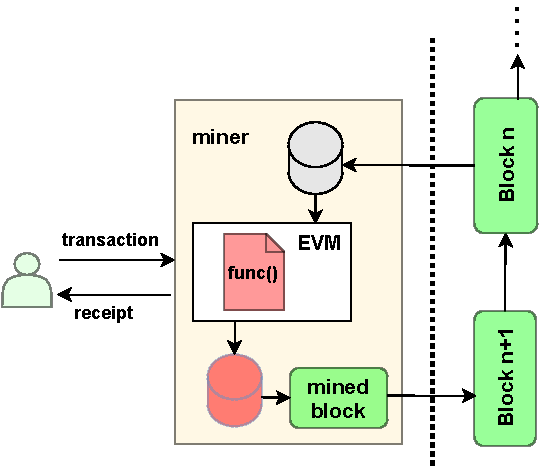
\includegraphics[scale=0.7]{Figures/Chapter5/SmartContractTransaction.pdf}
	\caption{The smart contract transaction on Ethereum.}
	\label{fig:smartcontractTransaction}
\end{figure}

A \emph{blockchain} is often called a distributed ledger recording transactions, consisting of blocks linked by cryptographic hashes and managed by a peer-to-peer network.
A blockchain can support not only transactions among users but also transactions between users and smart contracts.
\emph{Ethereum} is one of the most popular blockchains today, as it supports smart contracts~\cite{}.
A \emph{smart contract} is a piece of code that is executed autonomously on the blockchain; the execution of the code usually incurs a small fee, and a transaction executed by a smart contract may affect its own balance or the balance of another smart contract.
Figure~\ref{fig:smartcontractTransaction} briefly shows smart contract transaction on Ethereum.
A user (or client) sends a transaction to a miner for executing a specific contract function after block $n$.
The miner then reads the blockchain state database and runs on it the called function whose operation codes are interpreted by Ethereum virtual machine (EVM).
Later, the blockchain state database transitions and the miner will commit the new state database to a mined block that is appended as block $n+1$ after validation.
Finally, the user gets a receipt to confirm the transaction result including its status, event logs, ether transferred, as well as gas consumption.\footnote{Gas is the fee paid to the miner by transaction sender.}
If the transaction status indicates success, the state of contract will transition to new one. Otherwise, the contract state will remain unchanged.
\begin{definition}
	\textbf{Contract State and Transaction.} 
	A contract state $\delta$ can be defined by $<\mathit{Bal}, G\_\mathit{vars}>$ where $\mathit{Bal}\in N$ is the cryptocurrency balance owned by the contract, and $G\_\mathit{vars}$ comprises the values of all the storage variables managed by the contract.
	For simplicity, we define a transaction to smart contract as $t\leftarrow <\mathit{sender}, \mathit{value}, \mathit{func}, \mathit{status}>$, where $\mathit{sender}$ is an external account to invoke the contract's function $\mathit{func}$, and $\mathit{value}$ is the amount of attached ether correspondingly. 
	If the function invocation succeeds, $\mathit{status}$ is ``1''; otherwise, $\mathit{status}$ is ``0''. 
	Hereby, the transition types of a contract state can be formalized as (a) and (b).
	\begin{align*}
		(a)\quad\delta \xrightarrow[t.\mathit{status}=0]{t} \delta \quad \quad
		(b)\quad\delta \xrightarrow[t.\mathit{status}=1]{t} \delta^{'}
	\end{align*}
	In this paper, we focus on the transitions of type $(b)$ as the state of a smart contract is changed by them.
\end{definition}

\begin{definition}
	\label{def: contractmodel}
	\textbf{Contract Model.} 
	A contract model $\mathit{M}$ can be defined by $(\delta_0, F, \Delta, T)$ where $\delta_0 \in \Delta$ is initial state of contract, $f \in  F$ is a public function of contract and $T \subseteq \Delta \times F \times \Delta $ is transition function of contract state.
	As stated before, only successful function invocation can change contract state.
	Further, the reachability of function is decided by predicates over current contract state instead of its input. 
	For simplicity, every function can be implied by a boolean program: $f\implies Precondition(\Delta_1) \land StateChanges(\Delta_2)$,  where \textit{Precondition($\Delta_1$)} is a set of predicates related to check of global variables, i.e., state variables of contract and \textit{StateChanges($\Delta_2$)} is a set of assignments of global variables.
\end{definition}

Meanwhile, most smart contracts are designed as an organization for a social purpose, where users explicitly or implicitly play different roles 
when they participate in smart contract via transactions.
These smart contracts have been widely adopted in many areas including finance, gambling, exchanges, governance, property and etc..
For instance, the Ethereum Name Service (ENS) uses contracts to provide the auction service for users bidding the domains on Ethereum;
Dicether uses contracts to maintain houses for users' participation in gambling games;
while CryptoKitties uses contracts to organize blockchain stores for the exchange, breeding and siring of digital pets implemented as non-fungible tokens (NFTs). 
Therefore, it is critical to ensure smart contracts achieve the safety for the sake of the security of managed digital assets belong to users of different roles.